\subparagraph{Examples}

\paragraph{}
Slow (negligible Coriolis) fall on the surface of the Earth


\begin{center}
	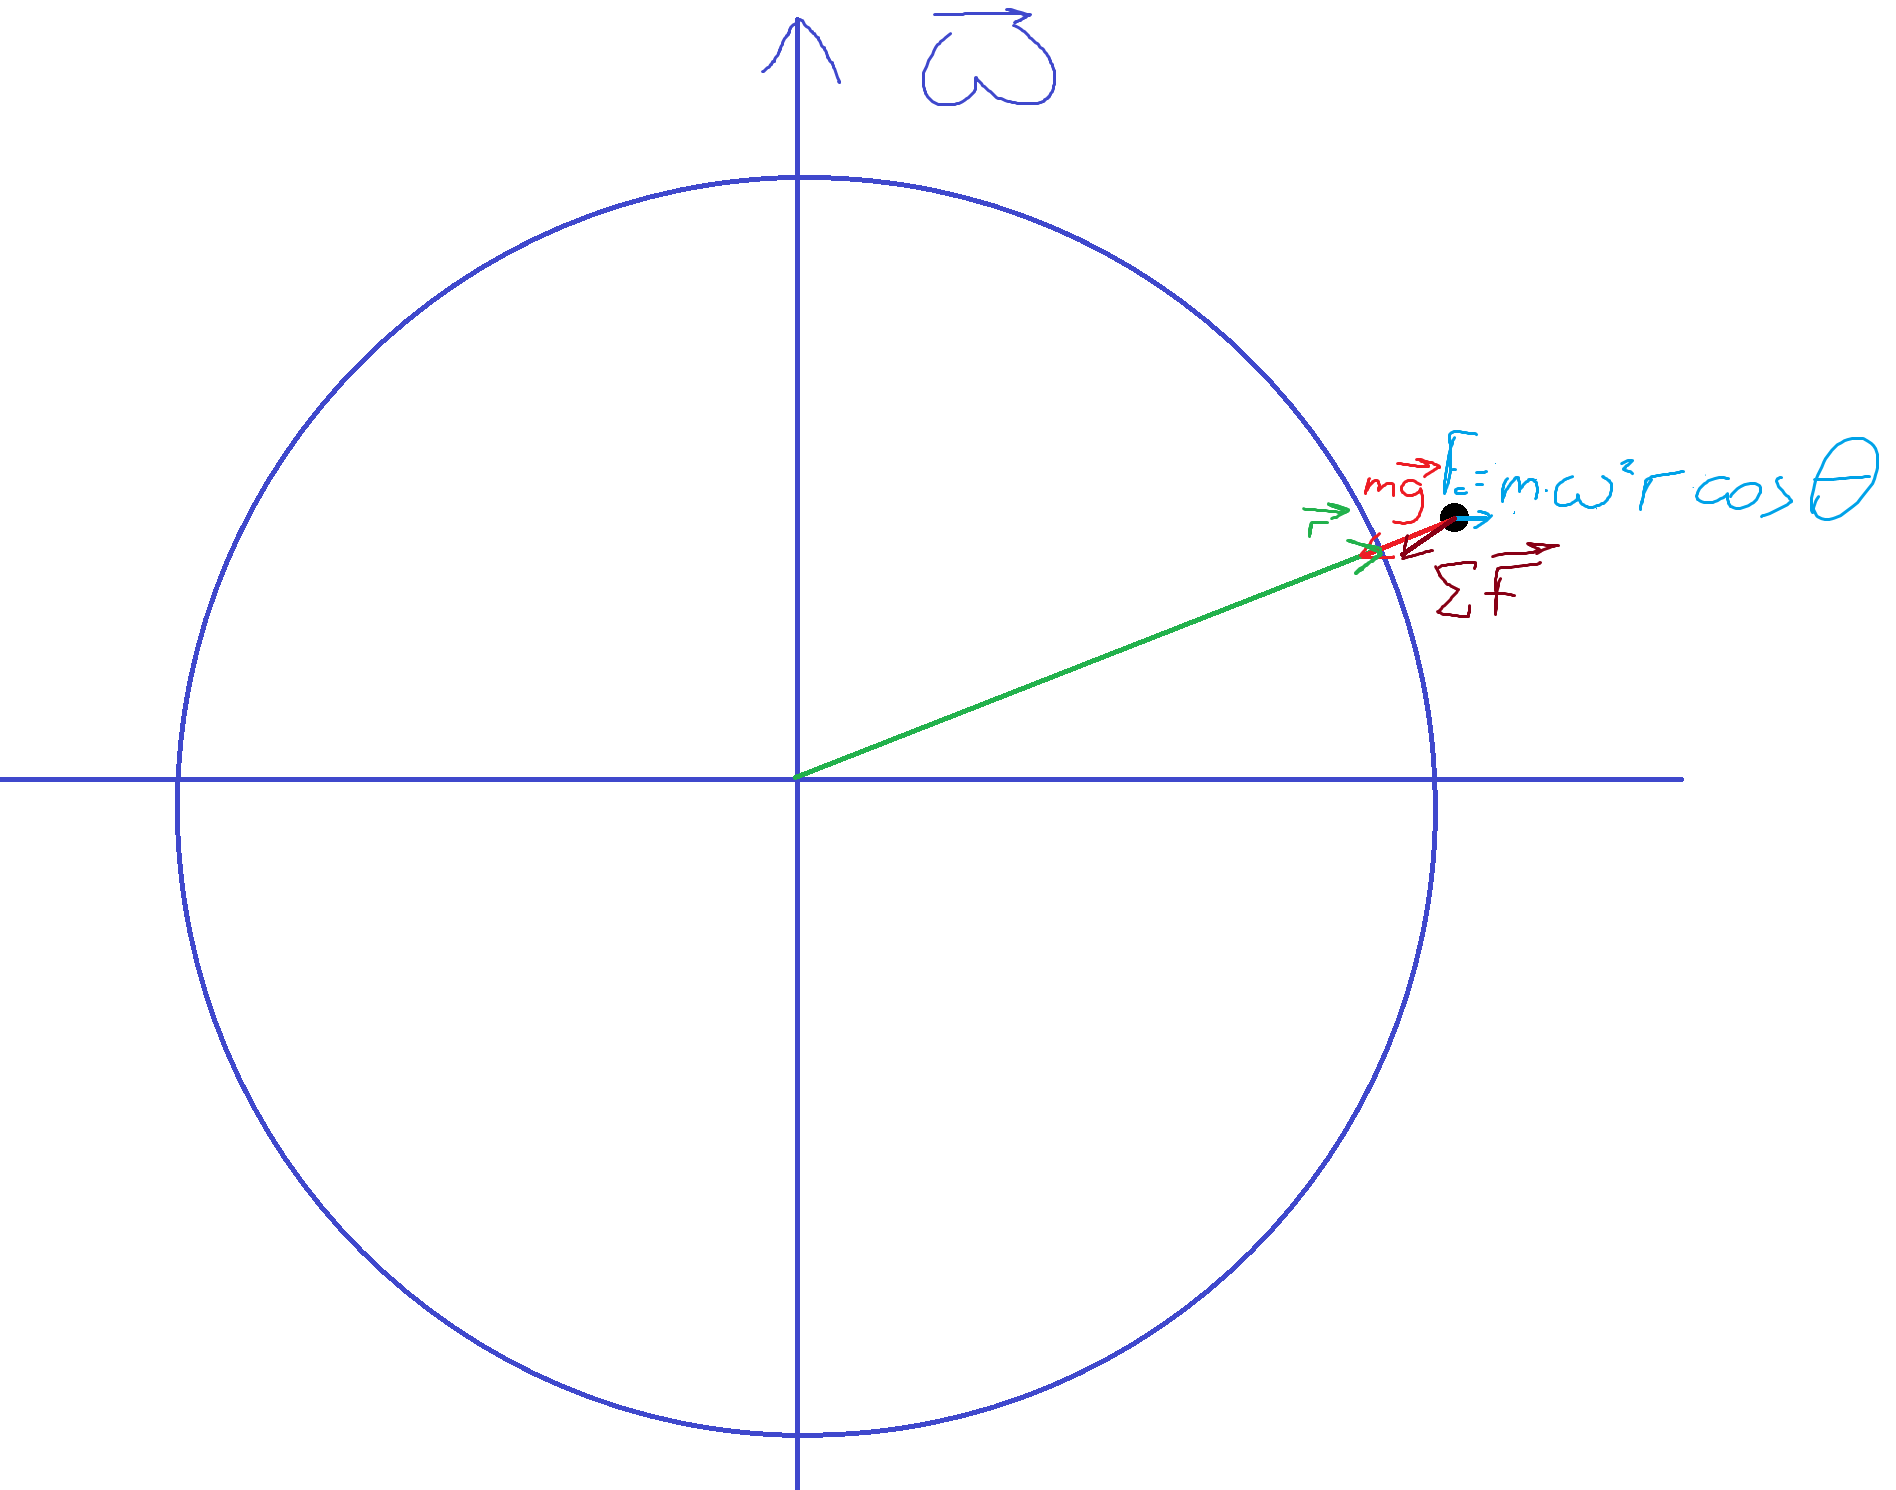
\includegraphics[width=\linewidth]{./lect8/pic1.png}
\end{center}

$$mg = 9.8m$$

Then centrifugal acceleration on equator equals to
$$a_c = \omega^2 r = \underbrace{\frac{2\pi}{\big[ (23 \cdot 60 +56) \cdot 60 \big]}}_{T_{turn}= 23 h 56 m} \cdot \underbrace{6.378 \cdot 10^6}_{Earth's \: radius} = 0.0339 ms^{-2}$$

\paragraph{}
Motion on Earth's surface (Coriolis).

\begin{enumerate}
	\item \begin{itemize}
		\item At the body moving to the East acts the force in direction $\hat{d}$ - out of rotational axis.
		
		\item At the body moving to the West acts the force in direction $\hat{d}$ - towards rotational axis.
	\end{itemize}
 
 
 
 \item \begin{itemize}
 	\item 
 	For horizontal motion in North hemisphere - Coriolis force's projection on the surface is to the right.
 	
 	\item 
 	For horizontal motion in South hemisphere - Coriolis force's projection on the surface is to the left.
 \end{itemize}
 



\item \begin{itemize}
	\item 
	
	At falling body acts Coriolis force to the East (at direction of rotation).
	
	\item 
	At rising body acts Coriolis force to the West.
\end{itemize}
\end{enumerate}

\paragraph{} Vertical throw.

Coriolis also changes the speed of the body, but while the velocity is low it's possible to neglect Coriolis velocity, i.e. $v_R=(v_0-gt)\hat{r}$ and the height will be $h = v_0 t - \frac{1}{2}gt^2$
$$a_{cor} = -2\vec{\omega} \times \vec{v}_R = 2 \left| \vec{\omega} \times \vec{v}_R  \right| = 2 \omega v_R \cos \lambda$$

Direction is to the West if $v_R>0$ else to the East.
If we denote by $+x$ direction to the West then:
$$\vec{a}_{cor} = 2 \omega v_R \cos \lambda \hat{x}$$

And 

$$\vec{v}_{cor} = \int \vec{a}_{cor} dt$$
$$\vec{x}= \int \vec{v}_{cor} dt$$

We can reduce the problem to 1 dimension and substitute $v_R$:
$$a_{cor} = 2 \omega (v_0 - gt) \cos \lambda$$

$$v_{cor} = \int_{0}^{t} 2 \omega (v_0 -gt^{\prime})dt^{\prime} \cos \lambda = 2 \omega \cos \lambda \int_{0}^{t}  \left(v_0 -gt^{\prime}\right) dt^{\prime} = 2 \omega \cos \lambda \left[  v_0 t^\prime - \frac{1}{2} gt^{\prime2}  \right]^t_0$$

$$v_{cor} = 2 \omega \cos \lambda \left(v_0t - \frac{1}{2}gt^2\right)$$

Now find deviation $x$:

$$\vec{x} = \int_0^{t_f} \vec{v}_{cor} dt$$

$$\vec{x} = 2 \omega \cos \lambda  \int_0^{t_f} \left(v_0t - \frac{1}{2}gt^2\right) dt =  2 \omega \cos \left[  \frac{1}{2}v_0 t^2 - \frac{1}{6}gt^{3}  \right]^{t_f}_0 $$

Since $t_F = \frac{2v_0}{g}$
$$\vec{x} = 2 \omega \cos \lambda  \left[ \frac{1}{2} v_0 \cdot \left( \frac{2v_0}{g} \right)^2 - \frac{1}{6}g \left(\frac{2v_0}{g}\right)^3 \right] $$

$$x = \frac{4}{3} \omega \cos \lambda \frac{v_0^3}{g^2}$$

\paragraph{Example} $v_0 = 200 ms^{-1}$, $\lambda=32\degree$

We get $h = 2040.8m \ll R_{Earth}$, then maximal $v_{cor} = 0.252 ms^{-1} \ll v_0$. We obtain deviation at return to the Earth's surface $x  = 6.85 m$

\section{Conservation of energy}

$$E_k = \frac{1}{2}mv^2$$ 

$$\vec{p}=m\vec{v}$$

\paragraph{} We start with one dimension $y$:

$$F = m \ddot{y}$$

Change in velocity is:

$$dv = \ddot{y}dt$$

If $v_0$ is initial velocity in $t=0$ then velocity at time $t$ is

$$\int_{v_0}^{v(t)} dv = \int_0^{t} \ddot{y} dt^\prime$$

$$v = \int_{0}^{t} \frac{F}{m} d t^\prime \stackrel{F=const}{=} \frac{F}{m}t$$

We do one more integral to get displacement:

$$y(t)-y_0 = \int_{0}^{t} v(t) dt^\prime = \int_{0}^{t} v_0 + \frac{F}{m}t^\prime dt^\prime = v_0t + \frac{1}{2}\frac{F}{m} t^2$$

From velocity equation we can get $t = \frac{m}{F}\left( v_t - v_0 \right)$ and then:

$$y-y_0 = \frac{1}{2}\frac{m}{F}\left( v^2 - v^2_0 \right)$$

By multiplying we acquire

$$\underbrace{F(y-y_0)}_{work} = \underbrace{\frac{1}{2}mv^2 - \frac{1}{2}mv_0^2}_{change \: in \: energy}$$